\section{Introduction}

Large language models (LLMs) are increasingly used as natural-language interfaces for querying tabular data. However, answering a query over a table requires more than understanding its wording: the model must recover the table structure, identify the cells that instantiate that structure, and perform the required operations. This is particularly challenging for non-relational tables, where the structure needed to answer the query is not represented by an explicit schema, but is encoded in the layout itself through hierarchical headers, merged cells, blank regions, noisy entries, or implicit dependencies between cells \cite{1.10}.

A large body of work has evaluated table reasoning through Table QA and Text-to-SQL benchmarks. Datasets such as Spider \cite{1.6}, BIRD \cite{1.20}, and BEAVER \cite{1.30} test whether models can generate executable SQL queries, including queries requiring joins across multiple relational tables. Because these benchmarks are public and widely used, however, evaluating recent LLMs on them raises contamination concerns \cite{datacontamination}. This has motivated automatically generated benchmarks, which extend semantic parsing resources through templated multi-table SQL generation \cite{?}, use database constraints to create automatically verifiable reasoning questions \cite{5.5}, or synthesize complex SQL programs over structured table--text collections \cite{5.8}. These approaches improve scalability and verifiability, but they inherit the structure of the underlying databases: schemas are explicit, join paths are known, and question complexity is bounded by the available relations. As a result, they provide limited control over whether the same query remains answerable when the latent data are fixed but the table presentation is perturbed. 
\fg1{This makes them less suited to answer the evaluation question targeted in this work: whether a model can recover the same latent evidence, perform the same operations, and produce the same answer when only the tabular presentation is systematically changed.}

\begin{figure}[t!]
    \centering
    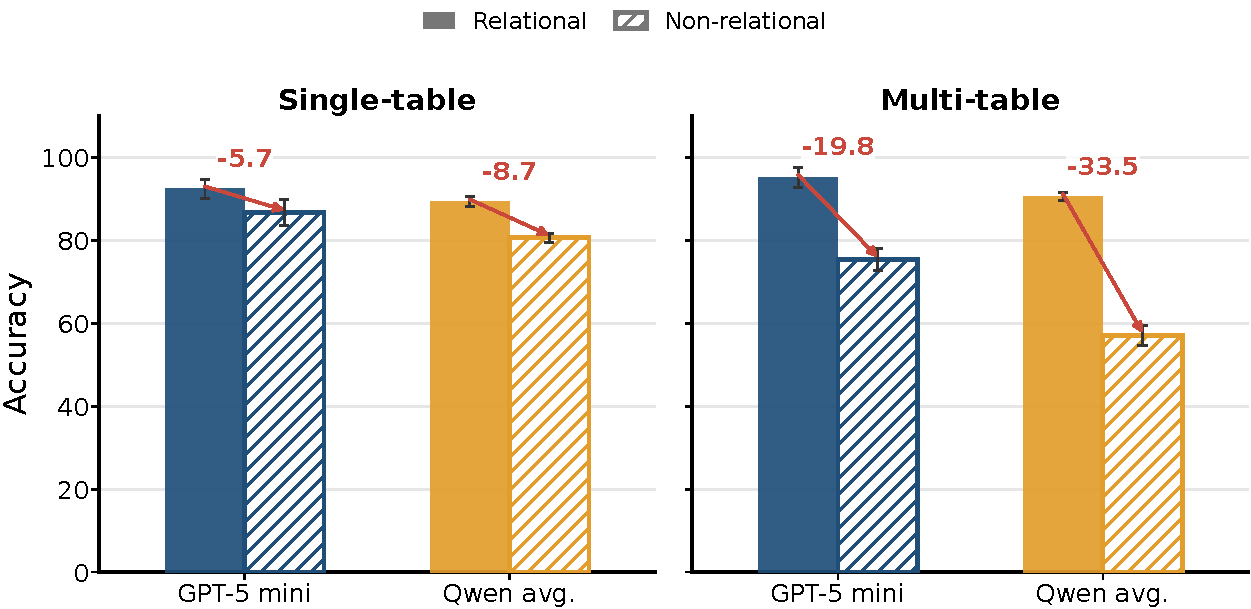
\includegraphics[width=0.48\textwidth]{img/rel_to_nonrel.pdf}
    \caption{Effect of non-relational perturbations on four databases extracted from Kaggle. Bars report absolute performance under relational and non-relational variants; red arrows indicate the corresponding drop. Non-relationalization consistently degrades performance, with substantially larger drops in the multi-table setting.}
    \label{fig:nonrelhurts}
\end{figure}

\begin{figure*}[t!]
    \centering
    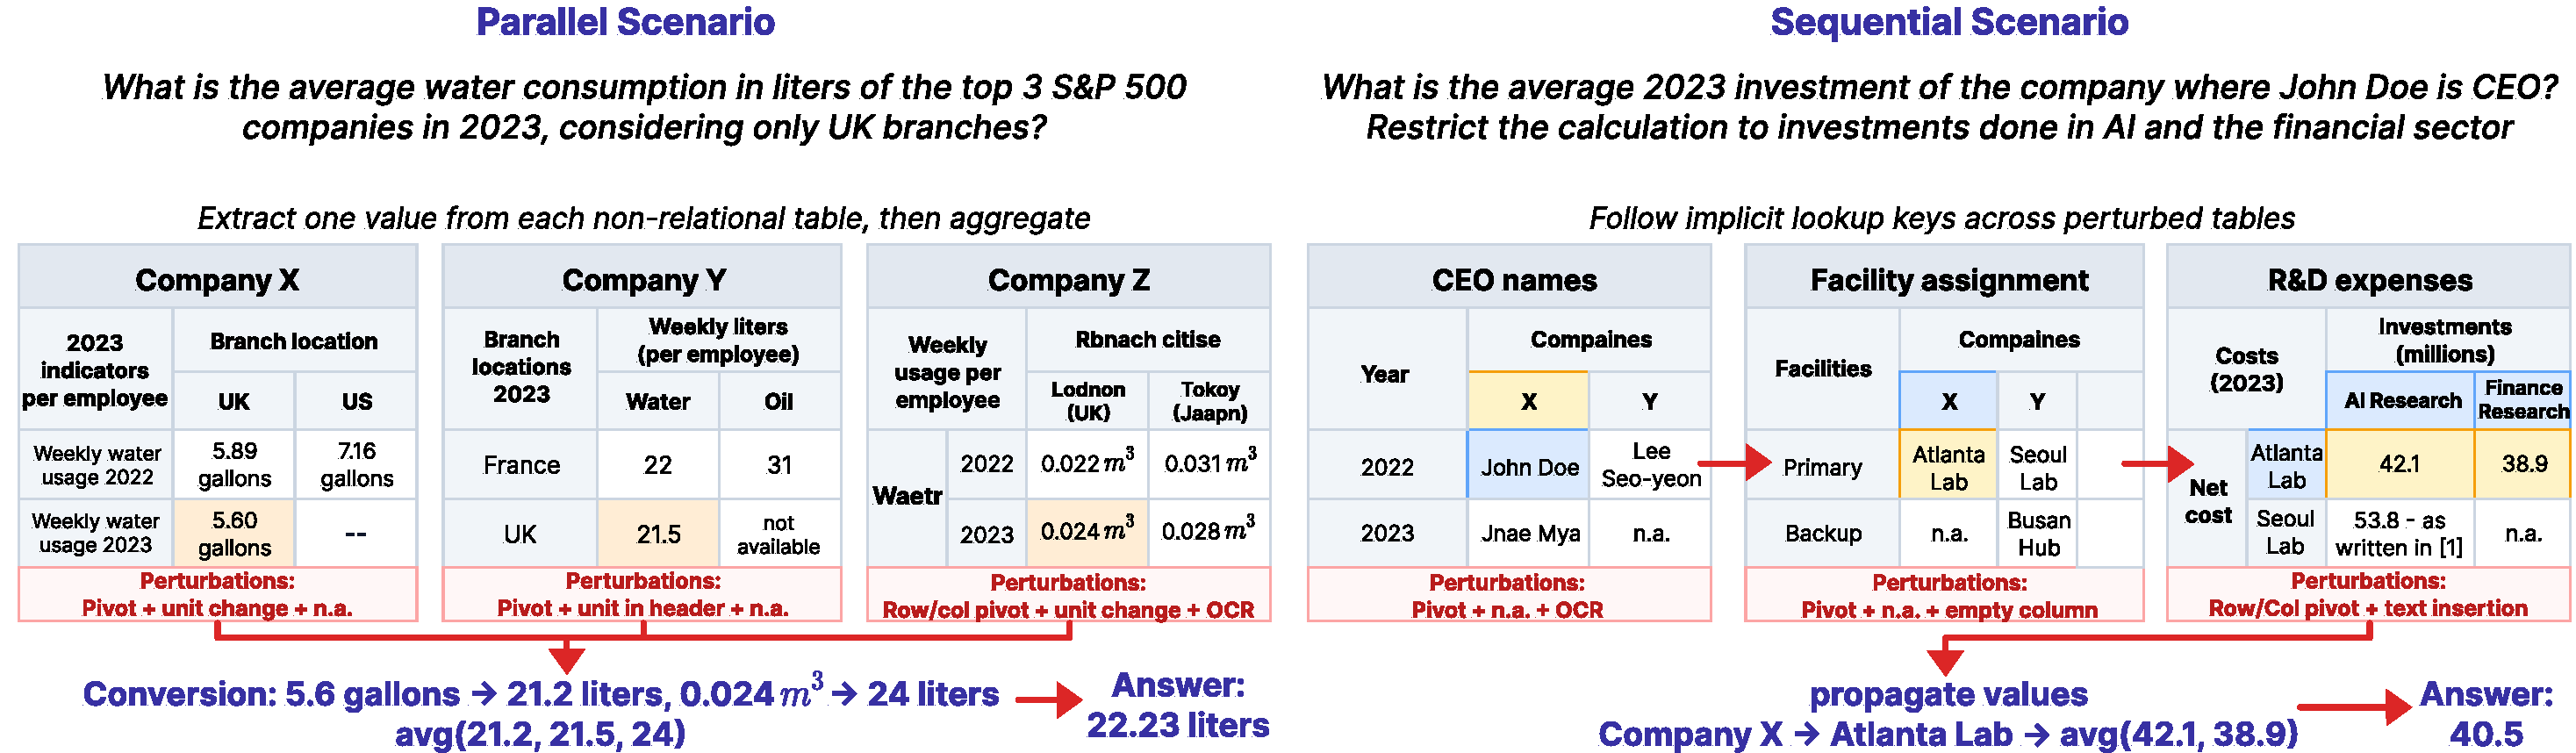
\includegraphics[width=0.99\textwidth]{img/q_types.pdf}
    \caption{Examples of parallel and sequential scenarios generated by \name over multiple non-relational tables. Parallel questions require extracting and aggregating values across perturbed tables, while sequential questions require propagating lookup keys across tables before aggregating the final values.}
    \label{fig:questiontypes}
\end{figure*}

This limitation is central for non-relational table reasoning. Layout changes, OCR-like noise, missing cells, and unit conventions can alter how evidence must be accessed without changing the gold answer. As shown in \autoref{fig:nonrelhurts}, even simple presentation changes reduce model performance, with substantially larger drops in the multi-table setting.

The multi-table setting amplifies this difficulty because models must not only interpret each perturbed table, but also decide how evidence should be combined across tables. This gives rise to two reasoning regimes. In \emph{parallel} reasoning, the model must extract comparable values from many independent tables and aggregate them, often after resolving differences in units or numerical conventions. In \emph{sequential} reasoning, the model must propagate intermediate entities or keys across tables, where links may be implicit and must be recovered through semantic matching rather than explicit foreign-key joins. \autoref{fig:questiontypes} illustrates both regimes: the parallel example requires extracting and normalizing one water-consumption value from each company table before averaging them, while the sequential example requires identifying a company from a CEO constraint, mapping it to its main lab, and aggregating the relevant R\&D investments. Such cases naturally arise in analytical queries; for example, asking for the average CO$_2$ emissions of all S\&P 500 companies may require reasoning over hundreds of distinct tables.

Evaluating this setting requires more than collecting difficult tables: the benchmark must control the number of tables, the reasoning regime, the perturbations applied to each table, and the gold answer after perturbation. A natural strategy is to start from existing relational datasets and transform them into non-relational views. In our experimental evaluation, however, we show that many tables from Spider, BIRD, and BEAVER cannot support the required layout perturbations or multi-table reasoning structures without invalid transformations or substantial manual intervention.

This motivates \name, a flexible \emph{from-scratch} benchmark generator for controlled evaluation of numerical question answering over multiple non-relational tables. \name is designed primarily as an evaluation framework: its goal is to generate automatically verifiable test instances in which the reasoning topology, number of tables, perturbation type, unit setting, and answer distribution can be controlled independently. Unlike prior work, \name~does not require an existing relational database, annotated examples, or manually curated source tables. Instead, a user specifies a target domain or topic and lightweight controls, such as the number of attributes, attribute cardinalities, number of tables, and unit settings. \name~then uses an LLM to generate a domain-specific schema, candidate attribute values, and semantic constraints, instantiates a \emph{latent relational source}, derives executable SQL supervision and scalar answers from it, and verbalizes the SQL programs into natural-language questions.

The key design choice is to separate supervision from presentation. The \emph{latent relational source} is used to compute answers, while models are evaluated on perturbed \emph{non-relational views}, i.e., table renderings generated by \name from the same latent source and shown to the model. This allows \name~to construct parallel and sequential multi-table regimes and to apply structural, cell-level, and unit perturbations, including pivots, nested headers, column merging, blank rows or columns, missing values, text insertions, typos, and unit changes, without changing the gold answer.

We evaluate \texttt{gpt-5-mini} and three \texttt{Qwen3.5} variants on financial and environmental instances generated by \name. Results show that performance decreases sharply as the number of tables increases, especially for parallel questions requiring many evidence values and sequential questions requiring implicit joins. We also find that unit perturbations have domain-dependent effects, suggesting that robust Table QA evaluation should account for both reasoning topology and domain-specific numerical conventions. Finally, although designed for controlled evaluation, \name can also provide useful supervision: fine-tuning on generated instances improves performance on GRI-QA \cite{1.16} compared to the non-finetuned Qwen baseline.

In summary, our contributions are threefold: 
(i) we introduce \name, a from-scratch generator for automatically verifiable numerical QA benchmarks over multiple non-relational tables; 
(ii) we define two controllable multi-table reasoning regimes, parallel and sequential, together with structural, cell-level, and unit-based perturbations that preserve answer correctness; 
(iii) we use \name to evaluate recent LLMs on financial and environmental domains, showing that non-relational perturbations, unit heterogeneity, and increasing numbers of tables substantially degrade performance. As an additional use case, we show that generated instances can also improve downstream Table QA training.